\chapter*{Introductie}
\addcontentsline{toc}{chapter}{Introductie}
In dit dictaat staat alle stof die je nodig hebt voor het vak Programmeren voor Dummies (2e jaar, kwartiel 4, opleiding Chemie). In dit vak wordt de programmeertaal Python gebruikt in combinatie met de software Pyzo om kennis te maken met programmeren. Het doel van het vak is dus niet om deelnemers binnen 4 weken vaardig te maken in programmeren, maar om in aanraking te komen met automatiseren en dataverwerken. 

Dit dictaat is geschreven in de taal \LaTeX met als editor \href{https://www.overleaf.com}{Overleaf}. 

Het vak is opgedeeld in 4 lessen.
\begin{itemize}
\item In de eerste les wordt de basis behandeld: hoe je code invoert en uitvoert, hoe je om input vraagt, en hoe je data op een simpele manier kan verwerken en kan laten zien. 
\item In de tweede les gaan we hier op verder en voegen we meer gereedschap toe om data te verwerken: loops, lijsten en functies. 
\item In de derde les leer je hoe je data uit een extern bestand kan ophalen en dit kan verwerken in bijvoorbeeld een grafiek. 
\item De laatste les is het uitvoeren van de eindopdracht van dit vak. 
\end{itemize}

Elke les bestaat uit een aantal verschillende onderwerpen. Per onderwerp zijn er een aantal oefeningen die je kunnen helpen met het begrijpen van de stof. Aan het einde van elk hoofdstuk staan een aantal opdrachten die testen of je de stof onder de knie hebt. De uitwerkingen van de opdrachten zijn beschikbaar. Houd er rekening mee dat als jouw antwoord net wat anders is, maar wel werkt, dit niet perse fout is. Er zijn vaak meerdere manieren om iets te programmeren.

Het dictaat is een onvolledige introductie tot Python. Python zelf heeft een uitgebreide tutorial (in het Engels) waar je alles kan vinden wat je nodig hebt, mocht het niet duidelijk worden uit het dictaat: \href{https://docs.python.org/3/tutorial/index.html}{https://docs.python.org/3/tutorial/index.html}. Handig om er naast te houden! Als je verder wil dan dit dictaat heeft de site datacamp.com erg goede tutorials en lesseries. Een aanrader is de volgende lesserie:
\href{https://www.datacamp.com/tracks/data-scientist-with-python}{Data scientist with Python}.

\textbf{Wat heb je nodig?}
\begin{itemize}
\item Een laptop met windows, MacOSX, of Linux
\item Dit dicaat
\item Een internetverbinding
\end{itemize}

Als je bovenstaande items hebt kan je starten aan dit vak. Voor het programmeren gebruiken we Pyzo, een gratis softwarepakket waar we in Python mee kunnen programmeren. Volg het onderstaande stappenplan om Pyzo te installeren.

Je kan ook met Python programmeren zonder iets te installeren. Je kan namelijk ook programmeren in je browser (Chrome, Firefox, wat dan ook). Je kan dat doen op de website \href{https://repl.it}{https://repl.it}. Maak een account aan, of log in met een bestaand account, en je kan gaan programmeren. Het is echter vaak handiger om Pyzo te installeren omdat je dan makkelijker kan werken met andere bestanden. Voor de eerste les maakt het niet veel uit.

LET OP: Het installeren van Pyzo duurt een tijdje, dus doe dat vantevoren! 

\textbf{Pyzo installeren}
\begin{itemize}
\item ga naar \href{http://www.pyzo.org/start.html}{http://www.pyzo.org/start.html}
\item Volg stap 1 t/m 3 (als stap 3 nog niet lukt: geen ramp!)
\end{itemize}

Als je Pyzo hebt geinstalleerd kan je aan de slag. Start het programma op. Je ziet als het goed is een scherm zoals in Fig.~\ref{fig:pyzokaal}.

\begin{figure}[h]
\begin{center}
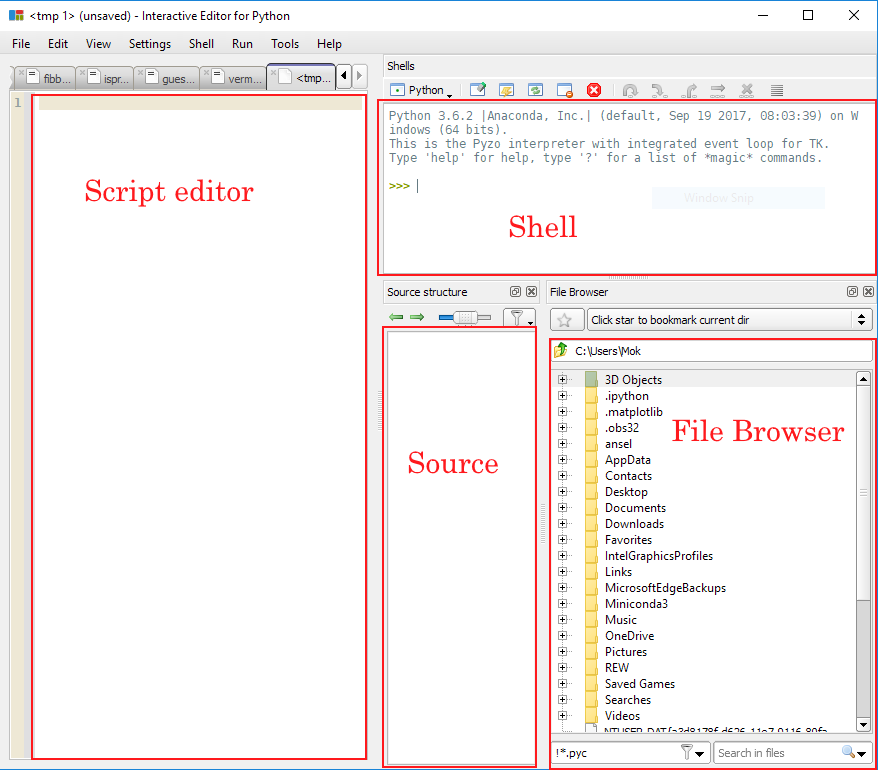
\includegraphics[width=0.6\textwidth]{img/pyzokaal.PNG}
\caption{\label{fig:pyzokaal} Pyzo zoals het eruit ziet als je het opstart. De rode text is later toegevoegd. }
\end{center}
\end{figure}

Dit is het hoofdscherm van Pyzo. Je ziet de volgende onderdelen:
\begin{itemize}
\item \textbf{Shell}: Dit is waar je output straks terecht komt, en waar je commando's in kan typen om uite voeren.
\item \textbf{Script Editor}: Dit is waar je langere code kan typen om op te slaan en te gaan draaien. Hierin werken we straks het meeste.
\item \textbf{Source}: Als je een groter, ingewikkeld programma hebt met meerdere bestanden zie je dat hier.
\item \textbf{File Browser}: Hier selecteer je in welke map je aan het werk bent.
\end{itemize}

In de Shell kan je dus code intypen om uit te voeren. Probeer het zelf: typ bijvoorbeeld in 5\texttt{+}8 en druk op enter. Wat je ook kan doen is je code in de Script Editor typen en dit script vervolgens uitvoeren. In les 1 gaan we hier mee bezig. In dit dictaat zullen voorbeelden worden gegeven van code, en dat ziet er als volgt uit:

\lstinputlisting{script/voorbeeld.py}

Je kan deze code kopieren in de Script Editor. Let wel op: Niet alles kopieert direct goed over. Let vooral op spaties, enters en tabs. Maak de code dus eerst netjes na het maken van de kopie.

Ga vervolgens naar Run -- Execute File om de code te draaien (of druk op CTRL-E). Als het goed is zie je dan de volgende output:
\begin{Verbatim}[frame=single]
>>> (executing file "<tmp 1>")
Hallo, chemicus!
13
Dit is het 0de nummer!
Dit is het 1de nummer!
Dit is het 2de nummer!
Dit is het 3de nummer!
Dit is het 4de nummer!
\end{Verbatim}

Als je een foutmelding krijgt heb je de code niet goed gekopieerd. Lees de foutmelding goed en zorg dat de code er exact hetzelfde uitziet als het voorbeeld! Als dit is gelukt ben je klaar om met het vak te beginnen.